\documentclass[20pt]{beamer}
\usepackage{beamerthemesplit}
\usepackage{apalike}
\usepackage{multirow}
\usepackage{rotating}
\usepackage{booktabs}
\usepackage{hyperref}
\usepackage{graphics}
\usepackage{microtype}
\usepackage{float}

%\newcommand{\mega}{\fontsize{100}{100}\selectfont}

\usetheme{boxes}
	\usecolortheme{seahorse}
%	\usecolortheme{dove}
													
%	Light
	%	\definecolor{LO}{RGB}{250, 162,  10}			
	%	\definecolor{LG}{RGB}{  9, 250, 162}		
	%	\definecolor{LP}{RGB}{162,	 9, 250}	

%	Dark
	%	\definecolor{DO}{RGB}{156, 100,   3}	
	%	\definecolor{DG}{RGB}{  2, 156, 100}
	%	\definecolor{DP}{RGB}{100,   2, 156}	
	
	
	\definecolor{LG}{RGB}{255, 213, 32}
	\definecolor{DG}{RGB}{ 0, 106, 83}
	\definecolor{DO}{RGB}{ 0, 106, 83}
	
\setbeamercolor{title}{fg=LG, bg=DO}		
\setbeamercolor{frametitle}{fg=LG, bg=DO}
\setbeamercolor{structure}{fg=DG}



\hypersetup{colorlinks, urlcolor=DG}
\hypersetup{colorlinks, linkcolor=DG}





\title[\texttt{R}]{Document Scraping and Text Analysis in \texttt{R}}
\author{\href{https://pds.ceu.hu/medzihorsky}{Juraj Medzihorsky}}
%\author{\href{https://pds.ceu.hu/medzihorsky}{\includegraphics[scale=0.15]{ja.png}}}
\institute{\href{http://www.ceu.hu}{
\includegraphics[scale=0.15]{CEU_logo_short.pdf}}
%\newline \href{http://www.fphil.uniba.sk/index.php?id=kpol}{
\includegraphics[scale=0.4]{logo_fak.png}}
}
\date{{\footnotesize{2014-11-03}}}

\begin{document}

\frame{\titlepage}


\begin{frame}
    \vspace*{-4mm}
	\hspace*{-5mm}
	\href{http://www.3ammagazine.com/3am/wp-content/uploads/2012/07/faust-33.jpeg}{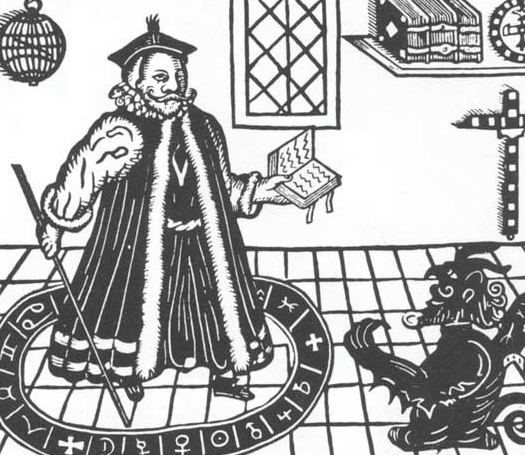
\includegraphics[height=1.05\paperheight]{faust-33.jpeg}}
\end{frame}


\begin{frame}
	\vspace*{-1mm}
	\hspace*{-12mm}
	\href{http://www.thegoodlifecentre.co.uk/wp-content/uploads/2012/05/IMG_1825.jpg}{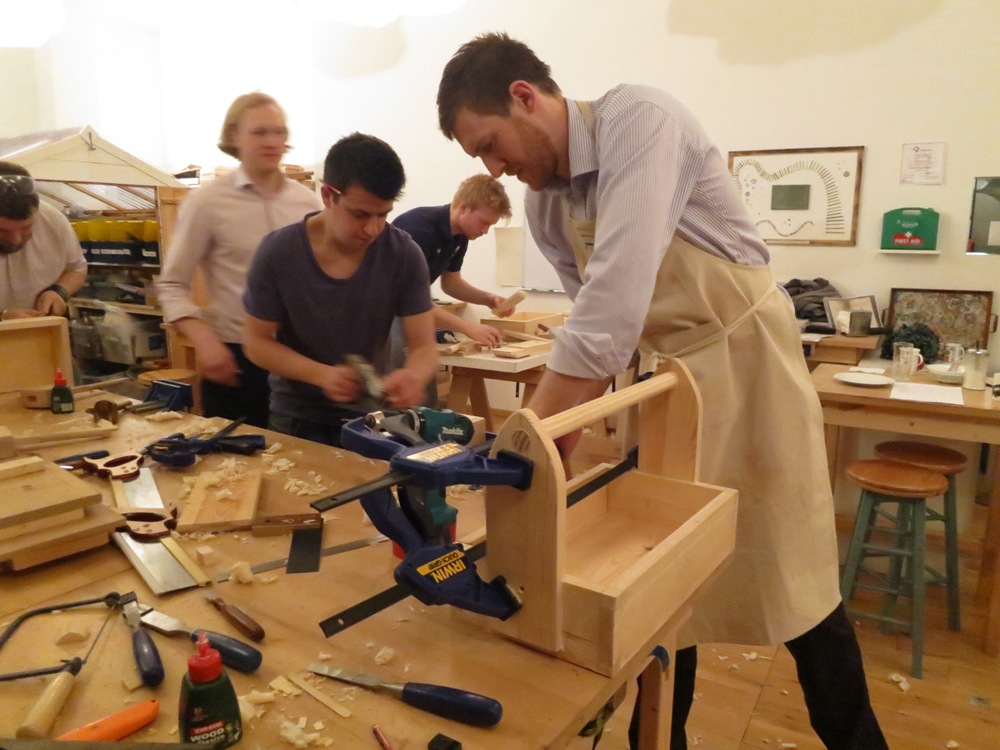
\includegraphics[height=1.1\textheight]{IMG_1825.jpg}}
\end{frame}


\begin{frame}
	\frametitle{Why \texttt{R}?}
	\begin{itemize}
		\item 	Free
		\item	Open source
		\item 	Large and diverse user community
		\item	Flexible
		\item 	Multi-platform
		\item 	Advanced: add-on packages, graphics
	\end{itemize}
\end{frame}


\begin{frame}{Community}
	\begin{itemize}
		\item Googling often more efficient than the \href{http://cran.r-project.org/manuals.html}{manuals}.
		\item Many specialized \href{http://www.r-project.org/mail.html}{mailing lists}.
		\item \href{http://stackoverflow.com/questions/tagged/r}{stackowerflow}
	\end{itemize}
\end{frame}


\begin{frame}{Graphics}
	\begin{itemize}
		\item 	Many options.
		\item	Many formats: vector vs. raster graphics.
	\end{itemize}
\end{frame}


\begin{frame}
	\frametitle{Vector vs. Raster Formats}
	\vspace*{-2mm}
%	\hspace*{-12mm}
%	
\href{http://kelseypromo.com/users/C7964980-844D-4673-BB99-4275098050BA/library/images/2259.gif}{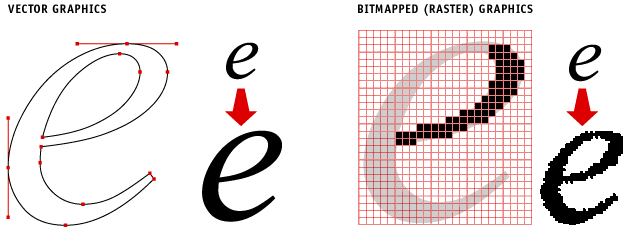
\includegraphics[width=1.0\textwidth]{2259.png}}
%
\end{frame}


\begin{frame}{Vector vs. Raster Formats}
	\begin{itemize}
		\item 	{\color{DG}Raster:} .jpg, .tiff, .png, .bmp ...
		\item	{\color{DG}Vector:} .pdf, .svg, .eps, .ppt ...
	\end{itemize}
\end{frame}



\begin{frame}
	\frametitle{How to use \texttt{R}?}
	\begin{itemize}
		\item 	{\bf{\color{DO}Directly:}} command line, console.
		\item	{\bf{\color{DO}GUI:}} default, \href{http://www.rstudio.com/}{RStudio}, \href{http://rforge.net/JGR/}{JGR}, \href{http://www.deducer.org/}{Deducer} etc.
		\item 	{\bf{\color{DO}Text editor + plugin:}}  \href{http://ess.r-project.org/}{Emacs}, \href{http://www.vim.org/scripts/script.php?script_id=2628}{vim}, \href{http://kevjohnson.org/using-r-in-sublime-text-3/}{Sublime Text} etc.
	\end{itemize}
\end{frame}


\begin{frame}
	\vspace*{-1mm}
	\hspace*{-12mm}
	\href{http://www.fler.cz/files/u/5/1/u5113/DSCN9921aaa.jpg}{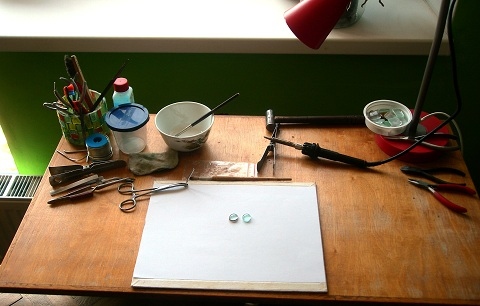
\includegraphics[height=1.1\textheight]{DSCN9921aaa.jpg}}
\end{frame}


\begin{frame}
	\frametitle{Workspace}
	\begin{itemize}
		\item 	Contains {\bf{\color{DG}objects}}
		\item 	List contents with {\tt ls()}
	\end{itemize}
\end{frame}


\begin{frame}
	\vspace*{-1mm}
	\hspace*{-12mm}
	\href{http://www.fler.cz/files/u/5/1/u5113/DSCN9921aaa.jpg}{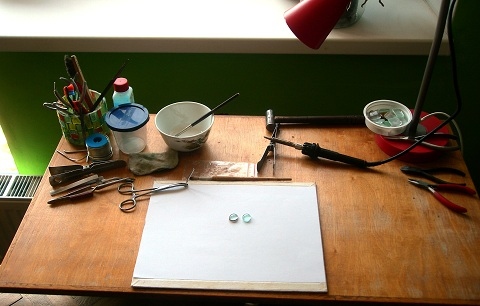
\includegraphics[height=1.1\textheight]{DSCN9921aaa.jpg}}
\end{frame}


\begin{frame}
	\frametitle{Objects}
	\begin{itemize}
		\item 	Data
		\item 	Functions
	\end{itemize}
\end{frame}


\begin{frame}
  \huge{	
  \begin{center}
	{\color{DG} Document Scraping}
  \end{center}
  }
\end{frame}


\begin{frame}
	\frametitle{Document Scraping}
	\begin{itemize}
		\item 	Numbers and text in files
		\item 	Local
        \item   Web 
	\end{itemize}
\end{frame}


\begin{frame}
    \vspace*{-4mm}
	\hspace*{-5mm}
	\href{http://www.3ammagazine.com/3am/wp-content/uploads/2012/07/faust-33.jpeg}{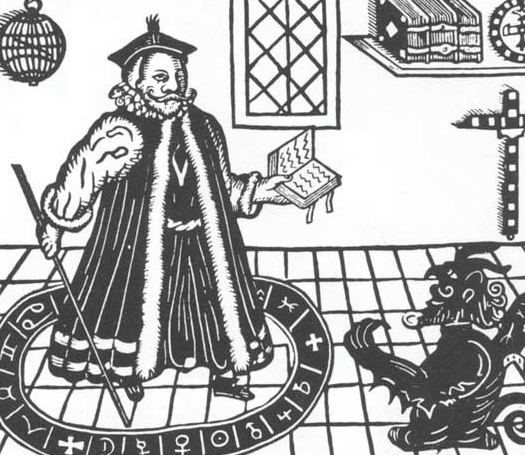
\includegraphics[height=1.05\paperheight]{faust-33.jpeg}}
\end{frame}


\begin{frame}
  \vspace*{-14mm}
  \begin{center}
	\href{http://bjws.blogspot.hu/2012/10/1930s-americas-great-depression-thomas.html}{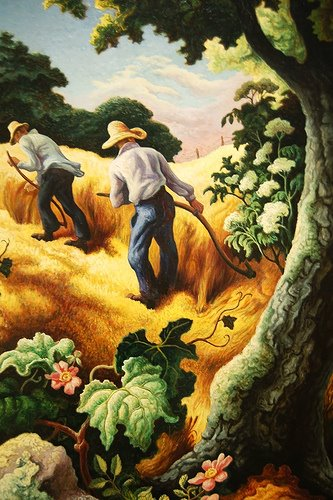
\includegraphics[height=1.5\paperheight]{jh.jpg}}
  \end{center}
\end{frame}


\begin{frame}
    \vspace*{-1mm}
    \hspace*{-12mm}
    \href{http://kombajnistibrezno.wbl.sk/zatva_zapad_2011.jpg}{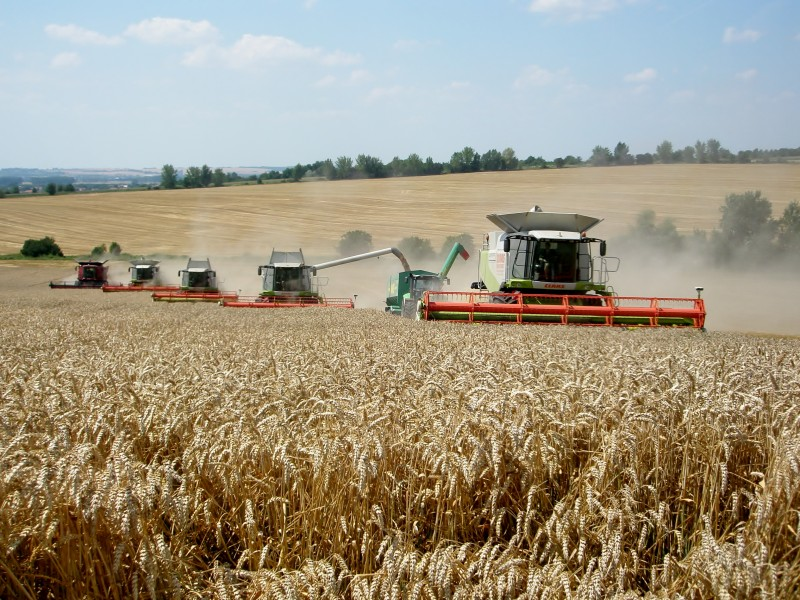
\includegraphics[width=1.01
\paperwidth]{zatva_zapad_2011.jpg}}
\end{frame}


\begin{frame}
	\frametitle{Web Scraping}
	\begin{itemize}
		\item 	HyperText Markup Language (HTML) familiarity
	\end{itemize}
\end{frame}



\begin{frame}
  \frametitle{}
  \begin{center}
    \href{http://www.clker.com/cliparts/5/9/3/4/11954357622059403819sheaf_john_olsen_01.svg.hi.png}{
\includegraphics[scale=1]{sheaf.png}}
        \end{center}
\end{frame}



\begin{frame}
  \huge{	
  \begin{center}
	{\color{DG} Text Analysis}
  \end{center}
  }
\end{frame}


\begin{frame}
	\frametitle{Text Analysis}
	\begin{itemize}
		\item 	Content Analysis
		\item 	`Manual' vs Computer Assisted Text Analysis (CATA)
	\end{itemize}
\end{frame}


\begin{frame}
	\frametitle{`Manual' Text Analysis}
	\begin{itemize}
		\item 	Humans do most of the work
		\item 	Expensive
        \item   Slow
        \item   Reliability issues 
	\end{itemize}
\end{frame}


\begin{frame}
	\frametitle{Computer Assisted Text Analysis}
	\begin{itemize}
		\item 	Computers do most of the work
		\item   Boom 
	    \begin{itemize}
		    \item 	Huge amount of digitized text available
            \item    Cheap computing power
            \item   New methods -- CS \& PS
     	\end{itemize}    
	\end{itemize}
\end{frame}


\begin{frame}
	\frametitle{`Bag of Words'}
	\begin{itemize}
		\item 	Common assumption in CATA
		\item 	Order of words (n-tuplets of words) does not matter
		\item 	Text as vector of word counts
	\end{itemize}
\end{frame}


\begin{frame}
	\frametitle{CATA in Political Science}
	\begin{itemize}
		\item Grimmer, J., \& Stewart, B. M. (2013). \href{http://pan.oxfordjournals.org/content/21/3/267}{Text as data: The promise and pitfalls of automatic content analysis methods for political texts}. {\it Political Analysis}, mps028.	
	\end{itemize}
\end{frame}


\begin{frame}
    \hspace*{-12mm}
    \href{http://pan.oxfordjournals.org/content/21/3/267}{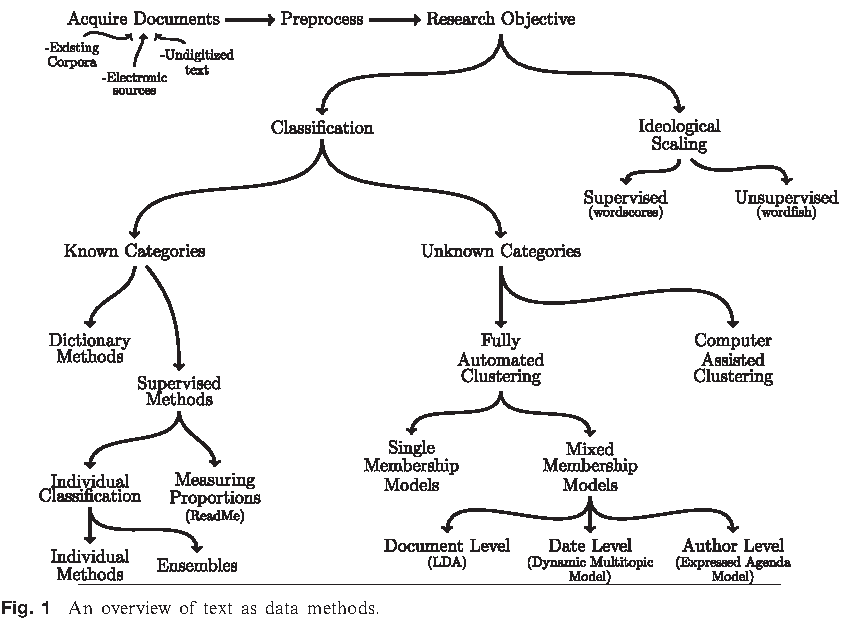
\includegraphics[width=\paperwidth]{gs_fig1_scissored.pdf}}
\end{frame}


\begin{frame}
	\frametitle{Scaling Goals}
	\begin{itemize}
		\item 	1 or more dimensions
		\item 	Place documents (texts, speeches) in space
		\item 	Place words in the same space
	\end{itemize}
\end{frame}


\begin{frame}
	\frametitle{Scaling Methods}
	\begin{itemize}
		\item 	Supervised: Wordscores
		\item 	Unsuperwised: Wordfish (1-factor Poisson IRT)
		\item 	Unsupervised: Correspondence Analysis
	\end{itemize}
\end{frame}


\begin{frame}
	\frametitle{Scaling Example 1}
	\begin{itemize}
		\item 	Republican presidential primaries for 2010 and 2014
		\item 	Transcripts of speeches from a UCSB website
		\item 	Expected move towards Tea Party positions
		\item   Wordfish
	\end{itemize}
\end{frame}

\begin{frame}
	\hspace*{-12mm}
    \href{http://journals.cambridge.org/action/displayAbstract?fromPage=online&aid=9365711&fileId=S1049096514001085}{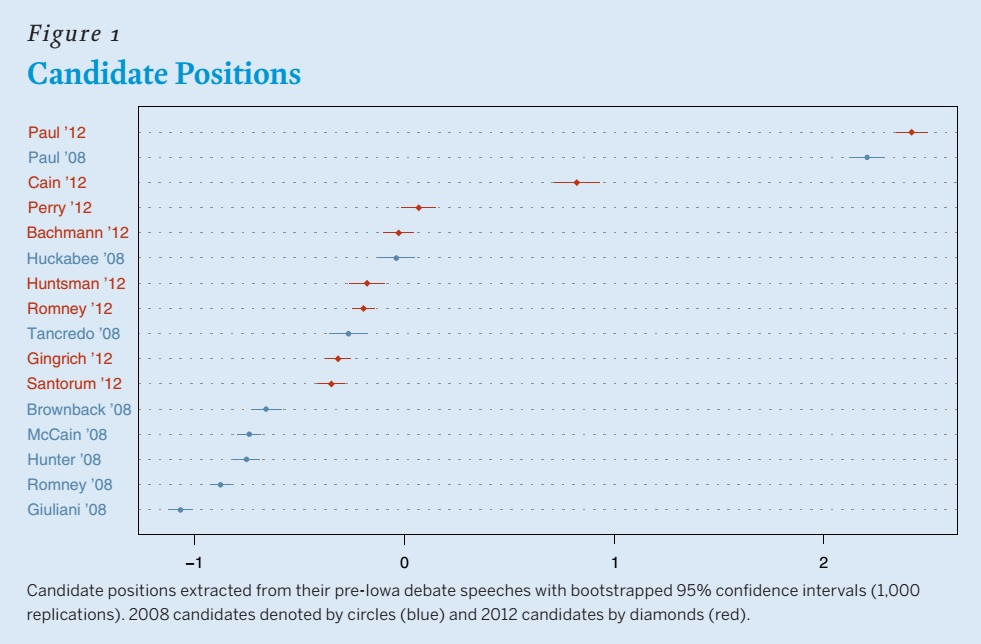
\includegraphics[width=1.01\paperwidth]{fig1_blog.jpg}}
\end{frame}


\begin{frame}
	\vspace*{-1mm}
	\hspace*{-12mm}
    \href{http://journals.cambridge.org/action/displayAbstract?fromPage=online&aid=9365711&fileId=S1049096514001085}{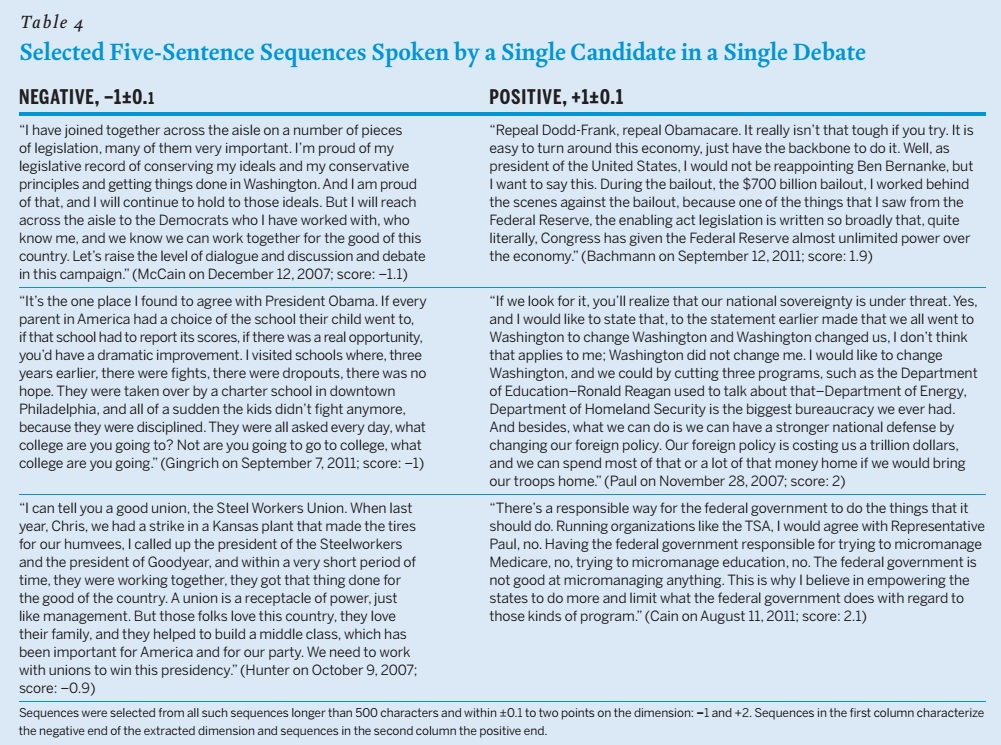
\includegraphics[width=1.01\paperwidth]{tab4_blog.jpg}}
\end{frame}


\begin{frame}
	\frametitle{Scaling Example 2}
	\begin{itemize}
		\item 	Fall of Radicova's gov't
		\item 	Transcripts of speeches from NRSR website
		\item 	Expected 2 dimensions: gov't support vs ESF support
		\item   Correspondence analysis
	\end{itemize}
\end{frame}


\begin{frame}
    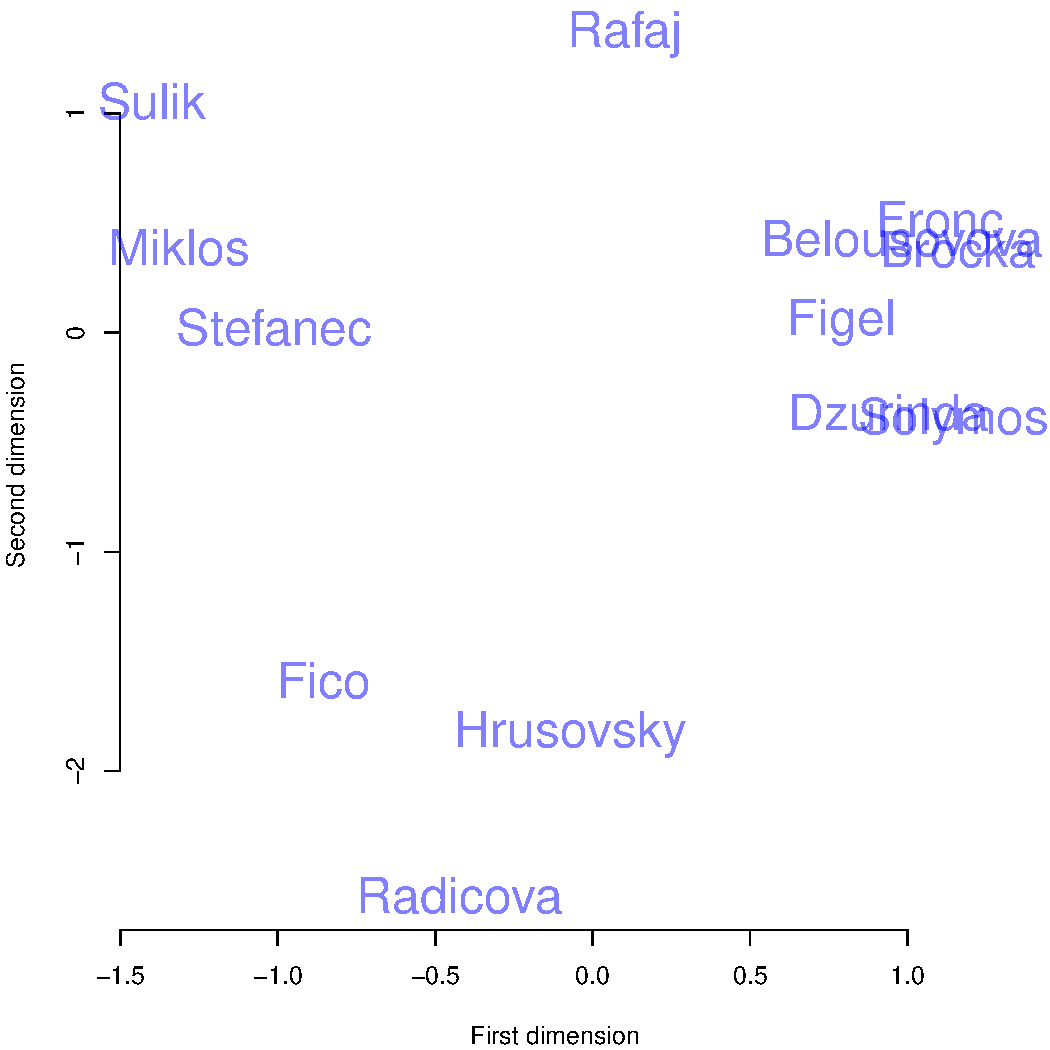
\includegraphics[width=\paperheight]{pv1.pdf}
\end{frame}


\begin{frame}
    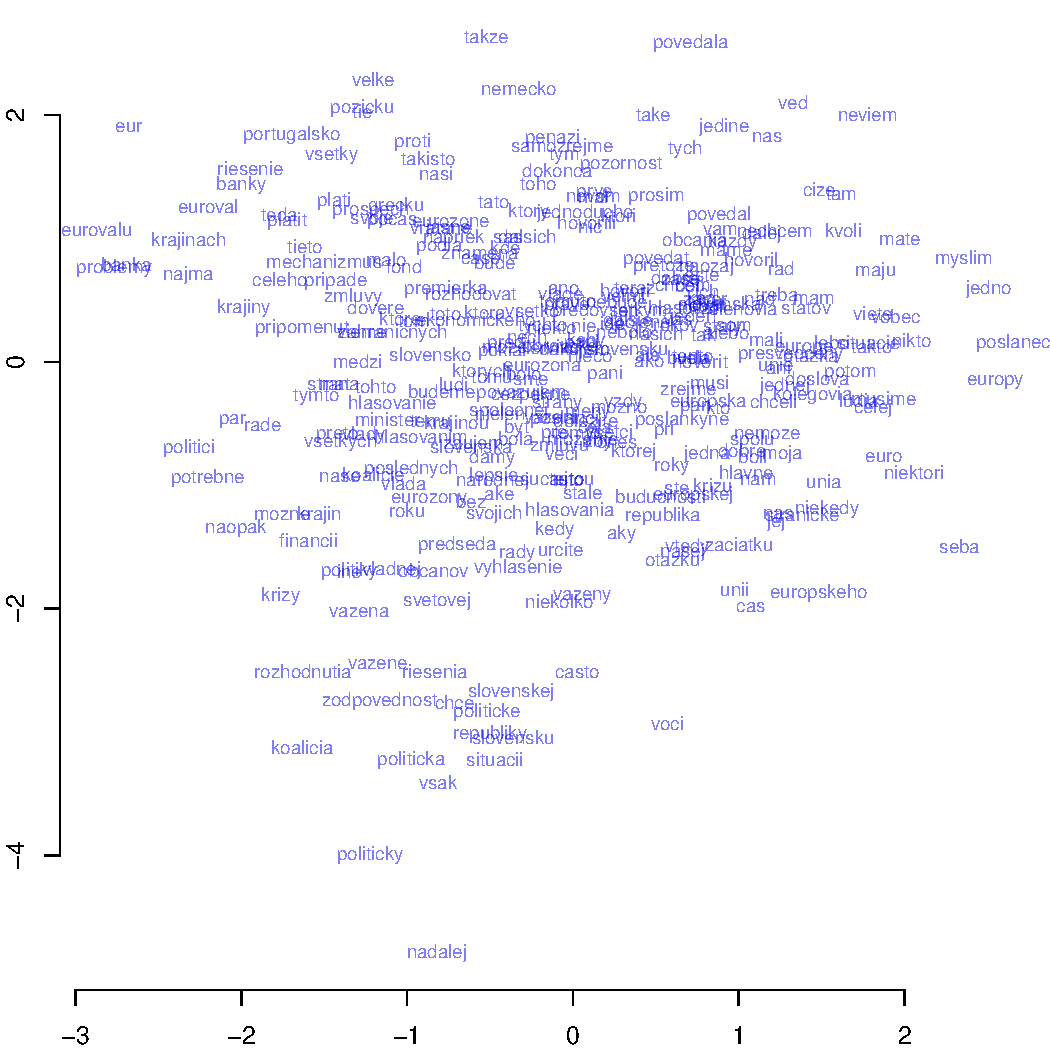
\includegraphics[width=\paperheight]{pv2.pdf}
\end{frame}


\begin{frame}
    \hspace*{-12mm}
    \href{http://pan.oxfordjournals.org/content/21/3/267}{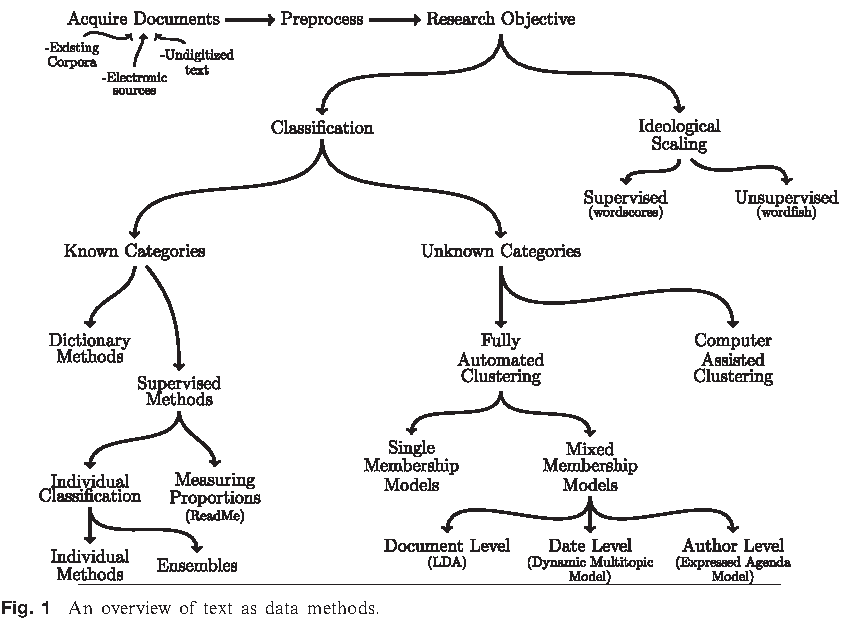
\includegraphics[width=\paperwidth]{gs_fig1_scissored.pdf}}
\end{frame}


\begin{frame}
	\vspace*{-1mm}
	\hspace*{-12mm}
	\href{http://www.thegoodlifecentre.co.uk/wp-content/uploads/2012/05/IMG_1825.jpg}{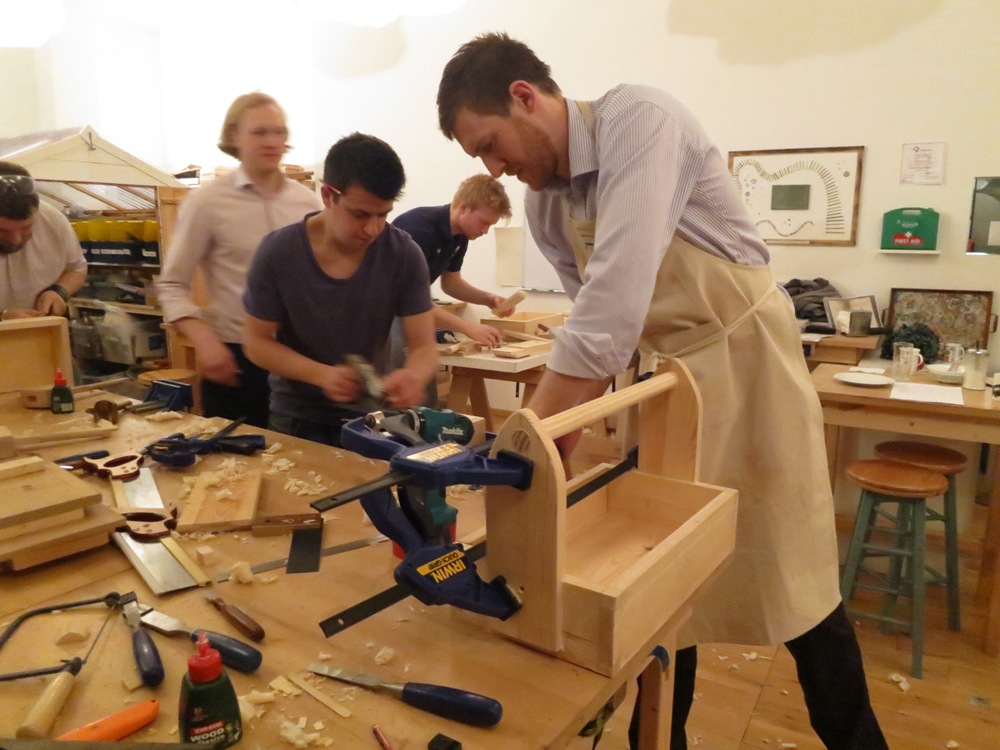
\includegraphics[height=1.1\textheight]{IMG_1825.jpg}}
\end{frame}


\end{document}
